\documentclass[article]{jss}

%% -- LaTeX packages and custom commands ---------------------------------------

%% recommended packages
\usepackage{thumbpdf,lmodern}

%% another package (only for this demo article)
\usepackage{framed}

%% Packages from FCVAR.m
\usepackage{amsmath}



%% new custom commands
\newcommand{\class}[1]{`\code{#1}'}
\newcommand{\fct}[1]{\code{#1()}}


%% -- Article metainformation (author, title, ...) -----------------------------

%% - \author{} with primary affiliation
%% - \Plainauthor{} without affiliations
%% - Separate authors by \And or \AND (in \author) or by comma (in \Plainauthor).
%% - \AND starts a new line, \And does not.
\author{Lealand Morin\\University of Central Florida
   \And Morten \O rregaard Nielsen\\Queen's University and CREATES
   \AND Micha\l{} Ksawery Popiel\\Analysis Group}
\Plainauthor{Lealand Morin, Morten \O rregaard Nielsen, Micha\l{} Ksawery Popiel}

%% - \title{} in title case
%% - \Plaintitle{} without LaTeX markup (if any)
%% - \Shorttitle{} with LaTeX markup (if any), used as running title
\title{The Fractionally Cointegrated Vector Autoregression Model in \proglang{R}}
\Plaintitle{The Fractionally Cointegrated Vector Autoregression Model in R}
\Shorttitle{FCVAR in \proglang{R}}

%% - \Abstract{} almost as usual
\Abstract{
  This article illustrates how to estimate 
  the fractionally cointegrated vector autoregression model in \proglang{R}.
}

%% - \Keywords{} with LaTeX markup, at least one required
%% - \Plainkeywords{} without LaTeX markup (if necessary)
%% - Should be comma-separated and in sentence case.
\Keywords{cofractional process, cointegration rank, fractional autoregressive model, fractional cointegration, fractional unit root, VAR model, \proglang{Matlab}, \proglang{R}}
\Plainkeywords{cofractional process, cointegration rank, fractional autoregressive model, fractional cointegration, fractional unit root, VAR model, Matlab, R}

%% - \Address{} of at least one author
%% - May contain multiple affiliations for each author
%%   (in extra lines, separated by \emph{and}\\).
%% - May contain multiple authors for the same affiliation
%%   (in the same first line, separated by comma).
\Address{
  Morten \O rregaard Nielsen\\
  Queen's University\\
  Address 1\\
  Address 2\\
  \emph{and}\\
  CREATES\\
  Address 1\\
  Address 2\\
  E-mail: \email{mon@econ.queensu.ca}\\
  URL: \url{https://mortens.webpage/~software/}
}

\begin{document}


%% -- Introduction -------------------------------------------------------------

%% - In principle "as usual".
%% - But should typically have some discussion of both _software_ and _methods_.
%% - Use \proglang{}, \pkg{}, and \code{} markup throughout the manuscript.
%% - If such markup is in (sub)section titles, a plain text version has to be
%%   added as well.
%% - All software mentioned should be properly \cite-d.
%% - All abbreviations should be introduced.
%% - Unless the expansions of abbreviations are proper names (like "Journal
%%   of Statistical Software" above) they should be in sentence case (like
%%   "generalized linear models" below).

\section[Introduction: Cointegration and fractional integration in R]{Introduction: Cointegration and fractional integration in \proglang{R}} \label{sec:intro}

%\begin{leftbar}
%The introduction is in principle ``as usual''. However, it should usually embed
%both the implemented \emph{methods} and the \emph{software} into the respective
%relevant literature. For the latter both competing and complementary software
%should be discussed (within the same software environment and beyond), bringing
%out relative (dis)advantages. All software mentioned should be properly
%\verb|\cite{}|d. (See also Appendix~\ref{app:bibtex} for more details on
%\textsc{Bib}{\TeX}.)
%
%For writing about software JSS requires authors to use the markup
%\verb|\proglang{}| (programming languages and large programmable systems),
%\verb|\pkg{}| (software packages), \verb|\code{}| (functions, commands,
%arguments, etc.). If there is such markup in (sub)section titles (as above), a
%plain text version has to be provided in the {\LaTeX} command as well. Below we
%also illustrate how abbrevations should be introduced and citation commands can
%be employed. See the {\LaTeX} code for more details.
%\end{leftbar}

The fractionally cointegrated vector autoregression model is an excellent model...



In \proglang{R} \citep{R}, contegration is performed by the \fct{function1} and \fct{function2} in the \pkg{pscl}
package \citep{Jackman:2015}. 


This \proglang{R} packages is based on the \proglang{Matlab} package \pkg{FCVARmodel.m}
with documentation in \cite{Nielsen2016} and \cite{Nielsen2013}. 


The next section describes the FCVAR model and the restricted models that can be estimated with this program. Section \ref{sec:main} describes the functioning of the main program, which is a replication of one of the tables of results in \cite{JNP2014}. Section \ref{sec:illustrations} describes another example program, which demonstrates some additional functionality of the software. Importantly, these are the only two files that would need to be changed to apply the program for other empirical analyses. 
% Section \ref{sec programs} describes how each of the major program files work (each in a separate subsection). 
% The Appendix contains a version change log.


%% -- Manuscript ---------------------------------------------------------------

%% - In principle "as usual" again.
%% - When using equations (e.g., {equation}, {eqnarray}, {align}, etc.
%%   avoid empty lines before and after the equation (which would signal a new
%%   paragraph.
%% - When describing longer chunks of code that are _not_ meant for execution
%%   (e.g., a function synopsis or list of arguments), the environment {Code}
%%   is recommended. Alternatively, a plain {verbatim} can also be used.
%%   (For executed code see the next section.)

% \section{Models and software} \label{sec:models}
\section{The fractionally cointegrated VAR model} \label{sec:fcvar}

%\begin{leftbar}
%Note that around the \verb|{equation}| above there should be no spaces (avoided
%in the {\LaTeX} code by \verb|%| lines) so that ``normal'' spacing is used and
%not a new paragraph started.
%\end{leftbar}

The fractionally cointegrated vector autoregressive (FCVAR) model was proposed in \cite{Johansen2008} and analyzed by, e.g., \cite{johniel2010,johansen2012likelihood}. For a time series $X_{t}$ of dimension $p$, the fractionally cointegrated VAR model is given in error correction form as
\begin{equation}
\Delta^{d}X_{t}= \alpha \beta^{\prime} \Delta^{d-b} L_{b} X_{t} + 
\sum_{i=1}^{k}\Gamma_{i}\Delta^{d}\ L_{b}^{i}X_{t}
+ \varepsilon_{t},
\label{vecm model}%
\end{equation}
where $\varepsilon_{t}$ is $p$-dimensional $i.i.d.(0,\Omega)$, $\Delta^{d}$ is the fractional difference operator, and $L_{b}=1-\Delta^{b}$ is the fractional lag operator.\footnote{Both the fractional difference and fractional lag operators are defined in terms of their binomial expansion in the lag operator, $L$. Note that the expansion of $L_{b}$ has no term in $L^{0}$ and thus only lagged disequilibrium errors appear in \eqref{vecm model}.} \cite{johansen2012likelihood} imposed two restrictions on the parameter space, $d\geq b$ and $d-b<1/2$, in their asymptotic analysis. However, these restrictions were relaxed in \cite{JN2018b,JN2018}.

Model \eqref{vecm model} includes the \cite{Johansen1995} CVAR model as the special case $d=b=1$; see \cite{JN2018}. Some of the parameters are well-known from the CVAR model and these have the usual interpretations also in the FCVAR model. The most important of these are the long-run parameters $\alpha$ and $\beta$, which are $p \times r$ matrices with $0 \leq r \leq p$. The rank $r$ is termed the cointegration, or cofractional, rank. The columns of $\beta$ constitute the $r$ cointegration (cofractional) vectors such that $\beta' X_t$ are the cointegrating combinations of the variables in the system, i.e.\ the long-run equilibrium relations. The parameters in $\alpha$ are the adjustment or loading coefficients which represent the speed of adjustment towards equilibrium for each of the variables. The short-run dynamics of the variables are governed by the parameters $\Gamma=(\Gamma _{1},\ldots ,\Gamma _{k})$ in the autoregressive augmentation.

The FCVAR model has two additional parameters compared with the CVAR model, namely the fractional parameters $d$ and $b$. Here, $d$ denotes the fractional integration order of the observable time series and $b$ determines the degree of fractional cointegration, i.e.\ the reduction in fractional integration order of $\beta'X_t$ compared to $X_t$ itself. These parameters are estimated jointly with the remaining parameters. This model thus has the same main structure as in the standard CVAR model in that it allows for modeling of both cointegration and adjustment towards equilibrium, but is more general since it accommodates fractional integration and cointegration.

In the next four subsections we briefly describe the accommodation of deterministic terms as well as estimation and testing in the FCVAR model.


\subsection{Deterministic terms}


%% -- Main Program ---------------------------------------------------------


\section{Main Program} \label{sec:main}


Estimating the fractionally cointegrated vector autoregression model works like this...

Here is an example of code:
\begin{Code}
glm(formula, data, subset, na.action, weights, offset,
  family = gaussian, start = NULL, control = glm.control(...),
  model = TRUE, y = TRUE, x = FALSE, ...)
\end{Code}


%\begin{leftbar}
%As the synopsis above is a code listing that is not meant to be executed,
%one can use either the dedicated \verb|{Code}| environment or a simple
%\verb|{verbatim}| environment for this. Again, spaces before and after should be
%avoided.
%
%Finally, there might be a reference to a \verb|{table}| such as
%Table~\ref{tab:overview}. Usually, these are placed at the top of the page
%(\verb|[t!]|), centered (\verb|\centering|), with a caption below the table,
%column headers and captions in sentence style, and if possible avoiding vertical
%lines.
%\end{leftbar}

%\begin{table}[t!]
%\centering
%\begin{tabular}{lllp{7.4cm}}
%\hline
%Type           & Distribution & Method   & Description \\ \hline
%GLM            & Poisson      & ML       & Poisson regression: classical GLM,
%                                           estimated by maximum likelihood (ML) \\
%Zero-augmented & Poisson      & ML       & Zero-inflated Poisson (ZIP),
%                                           hurdle Poisson \\
%               & NB           & ML       & Zero-inflated NB (ZINB),
%                                           hurdle NB \\ \hline
%\end{tabular}
%\caption{\label{tab:overview} Overview of various count regression models. The
%table is usually placed at the top of the page (\texttt{[t!]}), centered
%(\texttt{centering}), has a caption below the table, column headers and captions
%are in sentence style, and if possible vertical lines should be avoided.}
%\end{table}




%% -- Illustrations ------------------------------------------------------------

%% - Virtually all JSS manuscripts list source code along with the generated
%%   output. The style files provide dedicated environments for this.
%% - In R, the environments {Sinput} and {Soutput} - as produced by Sweave() or
%%   or knitr using the render_sweave() hook - are used (without the need to
%%   load Sweave.sty).
%% - Equivalently, {CodeInput} and {CodeOutput} can be used.
%% - The code input should use "the usual" command prompt in the respective
%%   software system.
%% - For R code, the prompt "R> " should be used with "+  " as the
%%   continuation prompt.
%% - Comments within the code chunks should be avoided - these should be made
%%   within the regular LaTeX text.

\section{Illustrations} \label{sec:illustrations}

For a simple illustration of the FCVAR...
The data can be loaded by
%
\begin{CodeChunk}
\begin{CodeInput}
R> data("quine", package = "MASS")
\end{CodeInput}
\end{CodeChunk}
%
and a basic frequency distribution of the response variable is displayed in
Figure~\ref{fig:quine}.

%\begin{leftbar}
%For code input and output, the style files provide dedicated environments.
%Either the ``agnostic'' \verb|{CodeInput}| and \verb|{CodeOutput}| can be used
%or, equivalently, the environments \verb|{Sinput}| and \verb|{Soutput}| as
%produced by \fct{Sweave} or \pkg{knitr} when using the \code{render_sweave()}
%hook. Please make sure that all code is properly spaced, e.g., using
%\code{y = a + b * x} and \emph{not} \code{y=a+b*x}. Moreover, code input should
%use ``the usual'' command prompt in the respective software system. For
%\proglang{R} code, the prompt \code{"R> "} should be used with \code{"+  "} as
%the continuation prompt. Generally, comments within the code chunks should be
%avoided -- and made in the regular {\LaTeX} text instead. Finally, empty lines
%before and after code input/output should be avoided (see above).
%\end{leftbar}

\begin{figure}[t!]
\centering
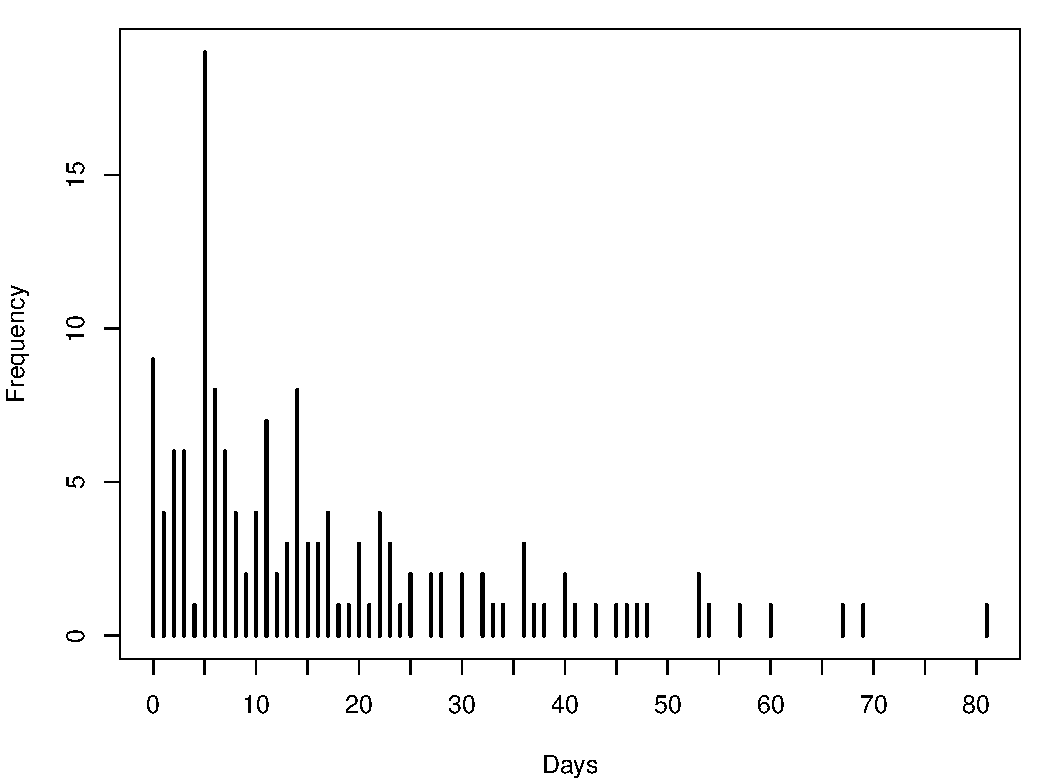
\includegraphics{delete-this-image}
\caption{\label{fig:quine} Frequency distribution for number of days absent
from school.}
\end{figure}

As a first model for the \code{quine} data, we fit the basic Poisson regression
model. (Note that JSS prefers when the second line of code is indented by two
spaces.)
%
\begin{CodeChunk}
\begin{CodeInput}
R> m_pois <- glm(Days ~ (Eth + Sex + Age + Lrn)^2, data = quine,
+    family = poisson)
\end{CodeInput}
\end{CodeChunk}
%
Hence, the full summary of that model is shown below.
%
\begin{CodeChunk}
\begin{CodeInput}
R> summary(m_nbin)
\end{CodeInput}
\begin{CodeOutput}
Call:
glm.nb(formula = Days ~ (Eth + Sex + Age + Lrn)^2, data = quine, 
    init.theta = 1.60364105, link = log)

Deviance Residuals: 
    Min       1Q   Median       3Q      Max  
-3.0857  -0.8306  -0.2620   0.4282   2.0898  

Coefficients: (1 not defined because of singularities)
            Estimate Std. Error z value Pr(>|z|)    
(Intercept)  3.00155    0.33709   8.904  < 2e-16 ***
SexM        -0.77181    0.38021  -2.030  0.04236 *  
EthN:AgeF2  -1.23283    0.42962  -2.870  0.00411 ** 
SexM:AgeF2   1.55330    0.51325   3.026  0.00247 ** 
SexM:AgeF3   1.25227    0.45539   2.750  0.00596 ** 
AgeF3:LrnSL       NA         NA      NA       NA    
---
Signif. codes:  0 '***' 0.001 '**' 0.01 '*' 0.05 '.' 0.1 ' ' 1

(Dispersion parameter for Negative Binomial(1.6036) family taken to be 1)

    Null deviance: 235.23  on 145  degrees of freedom
Residual deviance: 167.53  on 128  degrees of freedom
AIC: 1100.5

Number of Fisher Scoring iterations: 1


              Theta:  1.604 
          Std. Err.:  0.214 

 2 x log-likelihood:  -1062.546 
\end{CodeOutput}
\end{CodeChunk}



%% -- Summary/conclusions/discussion -------------------------------------------

%% -- Extensions ---------------------------------------------------------------------

\section{Extensions} \label{sec:extensions}

\subsection{Extension for $P$-values}


Although the Matlab program can run standalone, one of the functions, \verb|RankTests.m|, makes an external system call to a separately installed program, \verb|fdpval|. This external program is the C++ implementation of a Fortran program used to obtain simulated $P$-values from \cite{mackinnon2014numerical}. If the user would like $P$-values for the cointegration rank tests to be automatically calculated, we recommend obtaining this companion program, which is made available by Jason Rhinelander and can be downloaded from: 
\begin{center} \url{https://github.com/jagerman/fracdist/releases}
\end{center}
It can be either installed or downloaded in a compressed folder. It is important to note where the program is stored or installed, because the Matlab program requires the program location as an input in the estimation options. For example, if the program is stored in the folder \verb|/usr/bin/| on a Linux system, the location variable is defined as follows, \verb|progLoc = '"/usr/bin/fdpval"'|. For details see Sections~\ref{sec:estoptions.m} and~\ref{sec:getpvals}.

\subsection{Badly behaved objective function}

We also make use of the excellent \verb|extrema.m| and \verb|extrema2.m| functions, which are written by Carlos Adrián Vargas Aguilera and are freely available from the Mathworks website. For simplicity these are included in the Auxiliary subfolder.




%% -- Summary/conclusions/discussion -------------------------------------------

\section{Summary and discussion} \label{sec:summary}

Summary goes here. 


%% -- Optional special unnumbered sections -------------------------------------

\section*{Computational details}

%\begin{leftbar}
%If necessary or useful, information about certain computational details
%such as version numbers, operating systems, or compilers could be included
%in an unnumbered section. Also, auxiliary packages (say, for visualizations,
%maps, tables, \dots) that are not cited in the main text can be credited here.
%\end{leftbar}

The results in this paper were obtained using
\proglang{R}~3.4.1 with the
\pkg{MASS}~7.3.47 package. \proglang{R} itself
and all packages used are available from the Comprehensive
\proglang{R} Archive Network (CRAN) at
\url{https://CRAN.R-project.org/}.


\section*{Acknowledgments}

%\begin{leftbar}
%All acknowledgments (note the AE spelling) should be collected in this
%unnumbered section before the references. It may contain the usual information
%about funding and feedback from colleagues/reviewers/etc. Furthermore,
%information such as relative contributions of the authors may be added here
%(if any).
%\end{leftbar}

We are grateful to Federico Carlini, Andreas Noack Jensen, S\o ren Johansen, Maggie Jones, James MacKinnon, Jason Rhinelander, and Daniela Osterrieder for comments, and to the Canada Research Chairs program, the Social Sciences and Humanities Research Council of Canada (SSHRC), and the Center for Research in Econometric Analysis of Time Series (CREATES, funded by the Danish National Research Foundation DNRF78) for financial support.


%% -- Bibliography -------------------------------------------------------------
%% - References need to be provided in a .bib BibTeX database.
%% - All references should be made with \cite, \citet, \citep, \citealp etc.
%%   (and never hard-coded). See the FAQ for details.
%% - JSS-specific markup (\proglang, \pkg, \code) should be used in the .bib.
%% - Titles in the .bib should be in title case.
%% - DOIs should be included where available.

\bibliography{references}


%% -- Appendix (if any) --------------------------------------------------------
%% - After the bibliography with page break.
%% - With proper section titles and _not_ just "Appendix".

\newpage

\begin{appendix}

\section{More technical details} \label{app:technical}

%\begin{leftbar}
%Appendices can be included after the bibliography (with a page break). Each
%section within the appendix should have a proper section title (rather than
%just \emph{Appendix}).
%
%For more technical style details, please check out JSS's style FAQ at
%\url{https://www.jstatsoft.org/pages/view/style#frequently-asked-questions}
%which includes the following topics:
%\begin{itemize}
%  \item Title vs.\ sentence case.
%  \item Graphics formatting.
%  \item Naming conventions.
%  \item Turning JSS manuscripts into \proglang{R} package vignettes.
%  \item Trouble shooting.
%  \item Many other potentially helpful details\dots
%\end{itemize}
%\end{leftbar}

Technical details go here. 


%\section[Using BibTeX]{Using \textsc{Bib}{\TeX}} \label{app:bibtex}
%
%\begin{leftbar}
%References need to be provided in a \textsc{Bib}{\TeX} file (\code{.bib}). All
%references should be made with \verb|\cite|, \verb|\citet|, \verb|\citep|,
%\verb|\citealp| etc.\ (and never hard-coded). This commands yield different
%formats of author-year citations and allow to include additional details (e.g.,
%pages, chapters, \dots) in brackets. In case you are not familiar with these
%commands see the JSS style FAQ for details.
%
%Cleaning up \textsc{Bib}{\TeX} files is a somewhat tedious task -- especially
%when acquiring the entries automatically from mixed online sources. However,
%it is important that informations are complete and presented in a consistent
%style to avoid confusions. JSS requires the following format.
%\begin{itemize}
%  \item JSS-specific markup (\verb|\proglang|, \verb|\pkg|, \verb|\code|) should
%    be used in the references.
%  \item Titles should be in title case.
%  \item Journal titles should not be abbreviated and in title case.
%  \item DOIs should be included where available.
%  \item Software should be properly cited as well. For \proglang{R} packages
%    \code{citation("pkgname")} typically provides a good starting point.
%\end{itemize}
%\end{leftbar}

\end{appendix}

%% -----------------------------------------------------------------------------


\end{document}
